\documentclass{article}

\usepackage{amsmath, amsthm, amssymb, amsfonts}
\usepackage{thmtools}
\usepackage{graphicx}
\usepackage{setspace}
\usepackage{geometry}
\usepackage{float}
\usepackage{hyperref}
\usepackage[utf8]{inputenc}
\usepackage[english]{babel}
\usepackage{framed}
\usepackage[dvipsnames]{xcolor}
\usepackage{tcolorbox}
\usepackage{tikz}
\usepackage{multirow}
\usepackage{mathtools}

\colorlet{LightGray}{White!90!Periwinkle}
\colorlet{LightOrange}{Orange!15}
\colorlet{LightGreen}{Green!15}
\colorlet{LightBlue}{Blue!15}

\newcommand{\HRule}[1]{\rule{\linewidth}{#1}}
\DeclarePairedDelimiter\ceil{\lceil}{\rceil}

\declaretheoremstyle[name=Theorem,]{thmsty}
\declaretheorem[style=thmsty,numberwithin=section]{theorem}
\tcolorboxenvironment{theorem}{colback=LightBlue,arc=0mm}

\declaretheoremstyle[name=Proposition,]{prosty}
\declaretheorem[style=prosty,numberlike=theorem]{proposition}
\tcolorboxenvironment{proposition}{colback=LightOrange,arc=0mm}

\declaretheoremstyle[name=Principle,]{prcpsty}
\declaretheorem[style=prcpsty,numberlike=theorem]{principle}
\tcolorboxenvironment{principle}{colback=LightGreen,arc=0mm}

\declaretheoremstyle[name=Ejemplo,]{ejemplosty}
\declaretheorem[style=ejemplosty,numberwithin=section]{ejemplo}
\tcolorboxenvironment{ejemplo}{colback=LightGray, arc=0mm}

\setstretch{1.2}
\geometry{
    textheight=9in,
    textwidth=6.5in,
    top=1in,
    headheight=12pt,
    headsep=25pt,
    footskip=30pt
}

% ------------------------------------------------------------------------------

\begin{document}

% ------------------------------------------------------------------------------
% Cover Page and ToC
% ------------------------------------------------------------------------------

\title{ \normalsize \textsc{}
    \\ [2.0cm]
    \HRule{1.5pt} \\
    \LARGE \textbf{\uppercase{Programación Entera}
    \HRule{2.0pt} \\ [0.6cm] \LARGE{Apuntes de la asignatura} \vspace*{10\baselineskip}}
}

\author{\textbf{Autores} \\
    Juan Horrillo Crespo \\
    Universidad de Valladolid \\
    \date{\today}}

\maketitle
\newpage

\include{colaboraciones}

\tableofcontents
\newpage

% ------------------------------------------------------------------------------

\section{Problema de transporte}

\subsection{Introducción}
En este tema se estudiará el problema del transporte entre ciertos origenes y destinos. La característica común de los
modelos que se estudiarán es que los arrays\footnote{Estructura de datos que almacena una colección de elementos} resultantes 
serán completos, a diferencia de los arrays dispersos que se usarán en los problemas de flujos de redes.

\subsection{Descripción general}

El problema general del transporte se refiere a la distribución de bienes desde $m$ origenes (o centros de abastecimiento)
a $n$ destinos (o puntos de demanda) con el menor coste posible. Cada centro $i=1,\dots,m$ tiene asociado un coeficiente
$s_i$ que representa la oferta (cantidad máxima) que puede suministrar. Asi mismo, a cada punto demanda $j=1,\dots,n$ se
le asocia un coeficiente $d_j$ representando la cantidad requerida en dicho punto. Por último, asociado a cada ``trayectoria''
existe un coeficiente $c_{ij}$ que representa el coste por unidad de bien transportada desde el centro $i$ al punto $j$.

Definidos los coeficientes, el problema de transportes pretende suplir las demandas de los puntos desde los centros 
minimizando el coste total. Por tanto el planteamiento general es el siguiente

\begin{alignat}{3}
    \text{minimizar:}   & \quad & \sum^m_{i=1}\sum^n_{j=1}c_{ij}x_{ij}     & \quad &                        \label{eq:1}\\
    \text{sujeto a:}    & \quad & \sum^n_{j=1}x_{ij}\leq s_i               &       & \forall i=1,\dots,m    \label{eq:2}\\
                        & \quad & \sum^m_{i=1}x_{ij}\geq d_j               &       & \forall j=1,\dots,n    \label{eq:3}\\
                        & \quad & x_{ij}\geq 0                             &       & \forall i,j            \label{eq:4}
\end{alignat}

donde $x_{ij}$ representa la cantidad del bien transportado por la trayectoria que une el centro $i$ con el punto $j$.

\vspace*{2mm}

La función \ref{eq:1} se refiere al coste total del transporte. La restricción enunciada en \ref{eq:2} impide que se 
consuma más que la oferta ofrecida por un centro $i$. La restricción \ref{eq:3} es el equivalente para la demanda. Asegura
que se satisface la demanda en el punto $j$.

\vspace*{2mm}

Se considerará problema de transporte cualquier problema de programación lineal que tenga una forma análoga a la anterior,
sin necesariamente referirse a la distribución de algun bien.

\newpage

Para un problema de transporte se define la oferta total como la suma de las ofertas de cada centro, $O_T=\sum^m_{i=1}s_i$,
y la demanda total como la suma de las demandas de cada punto, $D_T=\sum^n_{j=1}d_j$. Se define un problema como de transporte 
balanceado cuando $O_T=D_T$. En caso de problema balanceado todas las restricciones (salvo la de no negatividad) se cumplen en
forma de igualdad, pudiendose reformular como

\begin{alignat}{3}
    \text{minimizar:}   & \quad & \sum^m_{i=1}\sum^n_{j=1}c_{ij}x_{ij}     & \quad &                        \\
    \text{sujeto a:}    & \quad & \sum^n_{j=1}x_{ij}= s_i                  &       & \forall i=1,\dots,m    \\
                        & \quad & \sum^m_{i=1}x_{ij}= d_j                  &       & \forall j=1,\dots,n    \\
                        & \quad & x_{ij}\geq 0                             &       & \forall i,j            
\end{alignat}

Cuando un problema no está balanceado, es facil convertirlo a uno que si. Cuando la oferta excede a la demanda total se 
añadirá un punto de demanda ficticio con demanda igual a la excedente de la oferta (como los envios a este punto no
se deben tener en cuenta, se asignará un coste 0). Estos puntos de demanda ficticios representan la oferta no usada, asi
pues, son las variables de holgura de las restricciones de oferta.

\noindent En caso de que la demanda sea mayor que la oferta ($D_T<O_T$), el problema no es factible.

\subsection{Obtención de soluciones factibles}

\begin{flushright}
    \textit{En lo que sigue, se consideran siempre problemas balanceados}
\end{flushright}

Un problema de transporte se puede representar en una tabla conocida como \textbf{tabla de transporte}

\begin{center}
    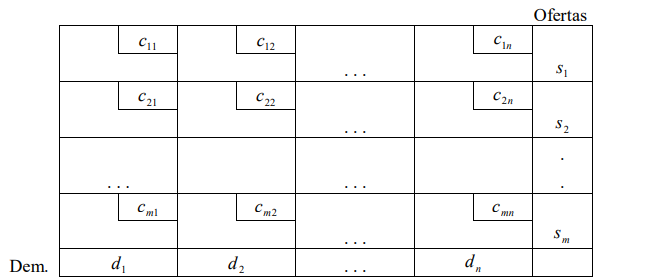
\includegraphics[width=0.9\textwidth]{img/TablaTransporte.png}
\end{center}

Dada una solución factible $X=(x_{1}|\cdots|x_{m})$ el valor asignado a cada variable $x_{ij}$ se sitúa en el interior
de la celda $ij$-ésima de la tabla. Todos los métodos de resoluciín que se ven utilizan esta tabla como base para la
realización de los cálculos. 

\newpage

\begin{itemize}
    \item \textbf{Método de la esquina noroeste}. Partimos de la tabla de transporte y comenzamos con la esquina superior
          izquierda (la que se encuentra más al ``noroeste''). A la variable $x_{11}$ se le asigna el máximo valor posible,
          esto es $min\{s_1, d_1\}$. Si se asigna $s_1$ esto significa que ningún otro punto podrá recibir el bien desde
          el primer centro, por lo que se tachan el resto de celdas de la fila y se sustituye $d_1$ por $d_1-s_1$. De
          forma análoga, si $x_{11}=d_1$ significa que se ha suplido toda la demanda del primer punto, por lo que se tachan
          el resto de celdas de la columna y se actualiza la cantidad de oferta $s_1-d_1$. Se repite el procedimiento 
          eligiendo de nuevo la próxima celda con el ``criterio noroeste'' entre las celdas disponibles (no tachadas) hasta
          que toda la demanda haya sido asignada.
    \item \textbf{Método greedy o de coste mínimo}. El anterior método no tiene en cuenta los costes de las trayectorias, por
          lo que a pesar de proporcionar una solución factible, rara vez se trata de la solución óptima. El procedimiento es
          el mismo pero cambia el criterio de selección de la celda, tomandose en cada iteración la celda de menor coste
          disponible.
    \item \textbf{Método de Vogel}. Para cada fila (columna) se calcula una penalización igual a la diferencia entre los dos 
          costes más pequeños de dicha fila (columna). Esta penalización indica el coste en el que se incurre por no elegir el 
          coste mínimo de dicha fila (columna). Se asigna el criterio de selección de celda a la menor penalización. En cada
          etapa se deben recalcular las penalizaciones. En caso de empate entre penalizaciones, se eligirá la del coste
          mínimo.
\end{itemize}

El método de coste mínimo puede (de casualidad) dar mejores resultados que el resto, pero por lo general el método de Vogel 
es el que genera una solución más cercana a la óptima, encontrando en ocasiones esta misma.

\subsection{Variantes del problema}

El problema de transportes general tiene numerosas variantes (o extensiones). Aquí se listan algunas de ellas

\begin{itemize}
    \item \textbf{Problemas no balanceados}. Ya hemos visto como se pueden formularse con igualdades.
    \item \textbf{Problemas de maximización}. En ocasiones se trata de maximizar una utilidad o un beneficio, siguiendo
          las restricciones típicas del problema de transporte. En este caso los criterios se deben tener en cuenta de 
          forma contraria, es decir, donde antes se buscaba el menor, ahora se busca el mayor.
    \item \textbf{Rutas prohibidas} (grafo no completo). En ocasiones no es posible enviar unidades desde el centro $i$
          al punto $j$. La forma más sencilla es considerar el problema como uno de redes, el cual simplemente elimina
          la variable $x_{ij}$. La segunda posibilidad es considerar el coste de la ``trayectoria'' muy elevado para que la
          variable $x_{ij}$ valga 0. Finalmente, otra tercera posibilidad es añadir la restricción  $x_{ij}=0$.
          \item \textbf{Caso capacitado}. En un problema de transporte con capacidades, se tienen las restricciones de cotas
          superiores para las variables de la forma $0\leq x_{ij}\leq u_{ij}$ para todas las rutas con capacidad. La 
          capacidad limita la cantidad del bien que puede ser enviada por una ``trayectoria'', por lo que se deben añadir
          estas restricciones cuando $u_{ij}<min\{s_i, d_i\}$ (no sería necesario añadirlas en caso contrario, pues ya 
          existen restricciones para $s_i$ y $d_i$).
\end{itemize}

\newpage

\subsection{Transporte Multiproducto}

En ocasiones, desde los centros de oferta, pueden salir distintos bienes o productos que pueden ser requeridos todos o algunos
de ellos desde los puntos de demanda. En este caso aumentan mucho los parámetros que intervienen en el problema. De forma
general consideraremos

\begin{center}
    \begin{tabular}{rcl}
        $m$         & = & número de puntos oferta \\
        $n$         & = & número de puntos demanda \\
        $p$         & = & número de productos ofertados y demandados \\
        $s_i^k$     & = & oferta del producto $k$ en el centro $i$ \\
        $d_j^j$     & = & demanda del producto $k$ en el punto $j$ \\
        $u_{ij}$    & = & cantidad máxima de flujo permitida en la ``trayectoria'' $ij$-ésima \\
        $c_{ij}^k$  & = & coste de transportar una unidad del producto $k$ del centro $i$ al punto $j$ \\
    \end{tabular}
\end{center}

El problema de encontrar la distribución de los productos con el mínimo coste posible se formula de la siguiente forma

\begin{alignat}{5}
    \text{minimizar:}   & \quad & \sum_{i,j,k}c_{ij}^kx_{ij}^k  & \quad &               \\
    \text{sujeto a:}    & \quad & \sum_{jk}x_{ij}^k\leq s_i^k   &       & \forall i,k   \\
                        & \quad & \sum_{ik}x_{ij}^k\leq d_i^k   &       & \forall j,k   \\
                        & \quad & \sum_kx_{ij}^k\leq u_{ij}     &       & \forall i,j   \\
                        & \quad & x_{ij}^k\geq 0                &       & \forall i,j,k           
\end{alignat}

donde $x_{ij}^k$ son las unidades del producto $k$ transportadas del centro $i$ al punto $j$.

\subsection{Transporte Multimodal}

En esta ocasión, pueden haber distintos modos de transporte (camión, tren, barco, \dots). También se puede tratar de 
distintas empresas o transportistas, cada una con su centro de distribución. De forma general (y para el caso de un único
producto) consideramos

\begin{center}
    \begin{tabular}{rcl}
        $m$         & = & número de puntos oferta \\
        $n$         & = & número de puntos demanda \\
        $p$         & = & número de modos de transporte \\
        $s_i$       & = & oferta en el centro $i$ \\
        $d_j$       & = & demanda en el punto $j$ \\
        $u_k$       & = & cantidad máxima que se puede distribuir por el medio de transporte $k$ \\
        $c_{ij}^k$  & = & coste de transportar del centro $i$ al punto $j$ mediante el transporte $k$ \\
    \end{tabular}
\end{center}

\newpage

El problema de encontrar la distribución del producto con el mínimo coste posible se formula de la siguiente forma

\begin{alignat}{5}
    \text{minimizar:}   & \quad & \sum_{i,j,k}c_{ij}^kx_{ij}^k  & \quad &               \\
    \text{sujeto a:}    & \quad & \sum_{jk}x_{ij}^k\leq s_i^k   &       & \forall i     \\
                        & \quad & \sum_{ik}x_{ij}^k\leq d_i^k   &       & \forall j     \\
                        & \quad & \sum_kx_{ij}^k\leq u_k        &       & \forall k     \\
                        & \quad & x_{ij}^k\geq 0                &       & \forall i,j,k           
\end{alignat}

donde $x_{ij}^k$ son las unidades del producto transportadas por el modo $k$ del centro $i$ al punto $j$.

\subsection{Producción-Distribución}

Se considera un problema en el que no solo hay costes de distribución, sino que se añaden los costos de producción, que
pueden ser diferentes en cada origen. Se desea conocer el nivel de producción que satisfaga las demandas sin superar
la capacidad de producción de cada centro y la distribución de la mercancía de forma que los costes totales sean mínimos. De
forma general consideraremos

\begin{center}
    \begin{tabular}{rcl}
        $m$         & = & número de fabricas o centros de producción \\
        $n$         & = & número de puntos demanda \\
        $s_i$       & = & capacidad de producción del centro $i$ \\
        $d_j$       & = & demanda en el punto $j$ \\
        $p_i$       & = & coste por unidad producida en la fabrica $i$ \\
        $u_k$       & = & cantidad máxima de flujo permitida en la ``trayectoria'' $ij$-ésima \\
        $c_{ij}$    & = & coste de transportar del centro $i$ al punto $j$ \\
    \end{tabular}
\end{center}

Si el problema está balanceado, quedará formulado de la siguiente forma

\begin{alignat}{3}
    \text{minimizar:}   & \quad & \sum^m_{i=1}\sum^n_{j=1}(c_{ij}+p_i)x_{ij}    & \quad &                        \\
    \text{sujeto a:}    & \quad & \sum^n_{j=1}x_{ij}= s_i                       &       & \forall i=1,\dots,m    \\
                        & \quad & \sum^m_{i=1}x_{ij}= d_j                       &       & \forall j=1,\dots,n    \\
                        & \quad & 0 \leq x_{ij} \leq u_{ij}                     &       & \forall i,j            
\end{alignat}

Si la oferta supera a la demanda se sustituyen las restricciones por ``menor o igual'' o ``mayor o igual'' teniendose en
cuenta de que las unidades producidas pero no distribuidas contribuyen con un coste igual al de su producción, o al de 
su producción y almacenamiento.

\newpage

\subsection{Dos etapas}

Es una extensión del problema de transporte que aparece frecuentemente. Suele ser necesario que existan almacenamientos
intermedios, que son puntos de transbordo donde no se acumula la mercancia (todo lo que entra sale). En general 
consideraremos

\begin{center}
    \begin{tabular}{rcl}
        $m$         & = & número de puntos oferta \\
        $n$         & = & número de puntos demanda \\
        $p$         & = & número de almacenes intermedios \\
        $s_i^k$     & = & oferta del en el centro $i$ \\
        $d_j^j$     & = & demanda del producto en el punto $j$ \\
        $c_{ik}^1$  & = & coste de transportar del centro de oferta $i$ al almacen $k$ \\
        $c_{ik}^1$  & = & coste de transportar del el almacen $k$ al punto $j$ \\
    \end{tabular}
\end{center}

Es posible modelizarlo de 3 formas distintas. Como un problema de transporte en dos etapas quedará formulado de la siguiente
forma

\begin{alignat}{6}
    \text{minimizar:}   & \quad & \sum^m_{i=1}\sum^n_{j=1}c_{ij}^1x_{ik}^1 + \sum^m_{i=1}\sum^n_{j=1}c_{ij}^2x_{kj}^2 & \quad &                        \\
    \text{sujeto a:}    & \quad & \sum^p_{k=1}x_{ik}^1\leq s_i  &               & \forall i=1,\dots,m           \\
                        & \quad & \sum^p_{k=1}x_{kj}^2\geq d_j  &               & \forall j=1,\dots,n           \\
                        & \quad & \sum^m_{i=1}x_{ik}^1 = \sum^n{j=1}x_{kj}^2    &       & \forall k=1,\dots,p   \\
                        & \quad & 0 \leq x_{ik}^1                               &       & \forall i,k           \\
                        & \quad & 0 \leq x_{kj}^2                               &       & \forall k,j
\end{alignat}

Como un problema de programación lineal con 3 índices

\begin{alignat}{3}
    \text{minimizar:}   & \quad & \sum^m_{i=1}\sum^p_{k=1}\sum^n_{j=1}(c_{ik}^1 + c_{kj}^2)x_{ikj}  & \quad &   \\
    \text{sujeto a:}    & \quad & \sum^p_{k=1}\sum^n_{j=1}x_{ikj}\leq s_i   &      & \forall i=1,\dots,m1       \\
    \text{sujeto a:}    & \quad & \sum^m_{i=1}\sum^p_{k=1}x_{ikj}\geq d_i   &      & \forall j=1,\dots,m        \\
                        & \quad & 0 \leq x_{ikj}                            &      & \forall i,k,j              \\
\end{alignat}

O como un progema de flujo en redes, que se verá en el proximo capitulo.

\vspace*{5mm}

\noindent Por supuesto, una restricción que se puede añadir en todos los anteriores ejemplos de formulación es la de 
capacidad de los almacenes $u_k$.
\section{Optimización en redes: El problema de flujo con coste mínimo}

\subsection{Introducción}

Los problemas de flujos en redes (tipo especial de los de transporte) permiten flujos que usan puntos intermedios o
de transbordo, y es característico el uso de arrays dispersos asociados a los arcos de un grafo no completo. Abarcan áreas
diversas como la producción, distribución y planificación de proyectos, localización de instalaciones, administración
de recursos y gestión de inversores entre otras. El problema más importante de optimización en redes es el problema de
flujo de costo mínimo.

\subsection{Terminología}

Un grafo consiste en un conjunto de puntos y un conjunto de líneas que unen unos pares de puntos. Siendo específicos, un
grafo está formado por \textbf{nodos} (los puntos) y \textbf{arcos o aristas} (las líneas). Por tanto, un grafo es un par
$(N,A)$ donde $N$ es un conjunto de nodos y $A$ un conjunto de arcos que relacionan los elementos de $N$. Un grafo puede
estar diseñado para permitir el paso de algún flujo, como puede ser la red de carreteras nacionales, un sistema de tuberías
o la block-chain (flujos de monedas entre carteras). Si el flujo se permite en una sola dirección se dirá que se trata de
un \textbf{arco dirigido}, en caso contrario será un \textbf{arco no dirigido}. Cuando una red solo tiene arcos no dirigidos
se habla de una \textbf{red dirigida} (como podráin ser las tuberías), así mismo y como se podría suponer, cuando una red
solo tiene arcos no dirigidos, se tratará de una \textbf{red no dirigida}. Toda red podrá considerarse dirigida sustituyendo
los arcos no dirigidos por un par de arcos dirigidos con direcciones opuestas.

\vspace*{2mm}

Una trayectoria entre dos nodos es la sucesión de arcos distintos que conectan ambos nodos. Cuando algunos o todos los
arcos de una red son arcos dirigidos, distinguiremos entre trayectorias dirigidas y trayectorias no dirigidas. Una 
\textbf{trayectoria dirigida o camino} del nodo $i$ al nodo $j$ es una sucesión de arcos cuya dirección es hacia el nodo 
$j$; de la misma forma, una \textbf{trayectoria no dirigida o cadena} del nodo $i$ al nodo $j$ es una sucesión de arcos
cuya dirección (si la tienen), es hacia o desde el nodo $j$.

\begin{center}
    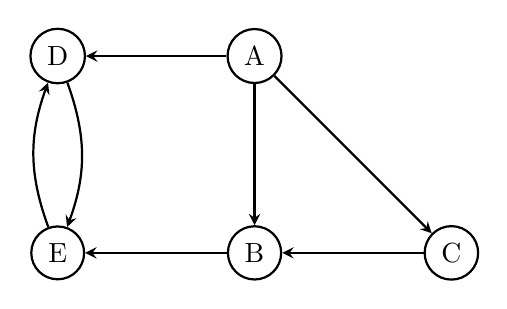
\begin{tikzpicture}[->, >=stealth, node distance=2.5cm, thick]
        % Nodos
        \node[circle, draw] (A) {A};
        \node[circle, draw, below of=A] (B) {B};
        \node[circle, draw, left of=B] (E) {E};
        \node[circle, draw, right of=B] (C) {C};
        \node[circle, draw, left of=A] (D) {D};
    
        % Aristas dirigidas
        \draw (A) -- (B);
        \draw (A) -- (C);
        \draw (A) -- (D);
        \draw (C) -- (B);
        \draw (B) -- (E);
        \draw[bend left=20] (D) to (E);
        \draw[bend left=20] (E) to (D);
    \end{tikzpicture}
\end{center}

Este grafo (red) está definidos por el conjunto de nodos $N=\{A,B,C,D,E\}$ y el conjunto de arcos 
$A={(A,B),(A,C),(A,D),(B,E),(C,B),(D,E),(E,D)}$. La sucesión de arcos $\{(C,B),(B,E),(E,D)\}$ es una trayectoria dirigida del
nodo $C$ al nodo $D$.

\newpage

\subsection{Problema del flujo de coste mínimo}

Sea $G=(N,A)$ un grafo dirigido con un conjunto de nodos $N=\{1,\dots,m\}$ y un conjunto de arcos $A$ representados por pares
$(i,j)$ con $i,j\in N$. La red corresponiende al grafo $G$ tiene los siguientes elementos adicionales.

\begin{itemize}
    \item Asociado a cada nodo $i\in N$ se tiene una cantidad $b_i$ que representa la oferta o demanda de cierto producto
          en ese nodo. Si $b_i>0$ se dice que el nodo es un \textbf{nodo oferta}, con un nivel de oferta (existencias o 
          producción) de $b_i$. Si $b_i<0$ entonces se dice que es un \textbf{nodo demanda}. Finalmente, si $b_i=0$ será
          un \textbf{nodo intermedio o de transbordo}.
    \item Para cada nodo $i\in N$ consideramos los conjuntos de nodos $\partial_i^+$ y $\partial_i^-$ donde 
          $\partial_i^+=\{j\in N:(i,j)\in A\}$ y $\partial_i^-=\{j\in N:(j,i)\in A\}$, representando al conjunbto de arcos
          ``salientes'' y ``entrantes'' respectivamente (a los que se llega desde $i$ y desde los que se llega a $i$).
    \item Asociado a cada arco una variable $x_{ij}\geq0$, que representa la cantidad de producto o flujo sobre el arco $(i,j)$
    \item Asi mismo, será $c_{ij}$ el coste por unidad del producto transportada a lo largo del arco.
    \item En ocasiones se establece $u_{ij}$ como la capacidad de flujo sobre el arco $(i,j)$.
\end{itemize}

\noindent La formulación del problema es la siguiente

\begin{alignat}{3}
    \text{minimizar:}   & \quad & \sum_{(i,j)\in A}c_{ij}x_{ij}                                     & \quad &                               \\
    \text{sujeto a:}    & \quad & \sum_{j\in \partial_i^+}x_{ij}-\sum_{j\in \partial_i^-}x_{ij}=b_i &       & \forall i\in N \label{eq:35}  \\
                        & \quad & x_{ij}\geq 0                                                      &       & \forall (i,j)\in A     
\end{alignat}

A las restricciones definidas en \ref{eq:35} se conocen como las \textit{ecuaciones de conservación de flujo}, 
\textit{ecuaciones de balance} o las \textit{ecuaciones de Kirchoff}. Hacen referencia al balance de los flujos de entrada
(aristas que vienen de los nodos $\partial_i^+$) y los flujos de salida (aristas que van a los nodos $\partial_i^-$) y el 
``consumo'' (o la ``emisión'') local definida por $b_i$.

\vspace*{2mm}

Si el número de arcos en el grafo es $n$ y representamos por $x=(x_{ij})$ al vector de variables o flujos, por $c=(c_{ij})$
al vector de costes y $b=(b_{i})$ el vector de ``balances'', el problema puede formularse de forma matricial como sigue

\begin{alignat}{3}
    \text{minimizar:}   & \quad & cx                & \quad &   \\
    \text{sujeto a:}    & \quad & Ax=b              &       &   \\
                        & \quad & x\geq \mathbf{0}  &       &        
\end{alignat}

donde $A$ es la matriz de coeficientes de las ecuaciones de balance. La variable $x_{ij}$ asociada al arco $(i,j)\in A$
aparecerá con coeficiente 1 en la restricción correspondiente al nodo $i$ y con coeficiente -1 en la restricción correspondiente
al nodo $j$. La matriz $A$ es conocida como \textit{matriz de incidencias nodos-arcos} para un grafo dirigido cualquiera.

\newpage

\begin{ejemplo}
    Para el grafo dado por el conjunto de nodos $N=\{1,2,3,4\}$ y el conjunto de arcos 
    $A=\{(1,2),(1,2),(2,3),(2,4),(3,2),(3,4),(4,1)\}$ la matriz de restricciones es la matriz de incidencias nodos-arcos

    \[A=\begin{pmatrix}
         1 &  1 &  0 &  0 &  0 &  0 & -1 \\
        -1 &  0 &  1 &  1 & -1 &  0 &  0 \\
         0 & -1 & -1 &  0 &  1 &  1 &  0 \\
         0 &  0 &  0 & -1 &  0 & -1 &  1
    \end{pmatrix}\]

    \noindent El arco $(1,2)$ une desde el nodo 1 al nodo 2, por lo que $a_{11}=1$ y $a_{12}=-1$, del mismo modo ocurre con 
    el resto de arcos. Como hay 4 nodos y 7 arcos las dimensiones de $A$ son $7\times 4$.
\end{ejemplo}

El modelo de flujos de redes tiene una propiedad importante, la \textbf{propiedad de integralidad} (no confundir con 
\textit{integrabilidad}). Esta propiedad puede enunciarse como ``si las ofertas y demandas son números enteros, toda solución
básica factible tiene valores enteros''. Es por esto que los problemas de flujo en redes muchas veces se incluyen en los
estudios del campo de la programación entera (como en nuestra asignatura).

\subsection{Redes balanceadas}

Se define la oferta total como la cantidad positiva $O_T=\sum_{b_i>0}b_i$, osea la suma de las ofertas. Del mismo modo,
se define la demanda total como la cantidad positiva $D_T=-\sum_{b_i<0}b_i$. Diremos que una red está balanceada si la oferta
es igual a la demanda, esto es $O_T=D_T$, o dicho de otra forma, si $\sum_ib_i=0$. Para todo problema factible su red está
balanceada, pero no toda red balanceada genera un problema factible.

\vspace*{2mm}

En muchos casos prácticos sucede que la oferta total no coincide con la demanda totaly es necesario ajustar el
problema para convertirlo en una red balanceada. Para ello se pueden asignar restricciones en función de si un nodo es de
oferta o de demanda, pero en la práctica esto resulta muy incomodo. Lo habitual es añadir un nodo ficticio conectado con arcos
dirigidos a todos los demás con coste 0 y demanda $D_T-O_T<0$

\subsection{Extensiones y aplicaciones}

En los problemas de redes, los costes y capacidades están siempre asociados a los arcos. En ocasiones, se quiere o necesita
establecer alguna de estas caracteristicas a un nodo (costes de fabricación, etc) por lo que se ha de crear un arco ficticio
que desdoble al nodo donde se adjudiquen estas características. Otra posible variante es incluir cotas mínimas, cambiando
las restricciones a $l_{ij}\leq x_{ij}\leq u_{ij}$.

\vspace*{2mm}

Existen otros problemas que generalizan el modelo básico y que tienen gran cantidad de aplicaciones en distintos sectores. A
pesar de que no se estudiarán, se enuncian algunos

\begin{itemize}
    \item Redes Generalizadas (tambien conocidas como Redes con Pérdidas y Ganancias)
    \item Redes Multiproducto
    \item Redes con costos fijos (se estudian en el tema de programación entera)
    \item Redes no lineales (cuando la función objetivo no es lineal)
\end{itemize}

Las aplicaciones más importantes de lo problemas de flujo en redes se dan en \textit{problemas de distribución}, pero tienen
impacto en ambitos como la planificación de \textit{redes espacio/tiempo} para modelizar problemas de producción/inventario.
\section{Programación Entera}

\subsection{Introducción}

Un problema de \textbf{Programación Lineal Entera} (PLE) es un problema de optimización de una función lineal en presencia
de restricciones lineales con la condición añadida de que alguna o todas las variables deben ser enteras. Cuando todas las
variables están obligadas a ser enteras entonces se habla de un problema de \textbf{Programación Entera Pura} y si solo son
algunas será un problema de \textbf{Programación Entera Mixta}. En ocasiones las variables enteras están limitadas a tomar
valores 0 o 1, a estas variables las denominaremos binarias. Si esta condición es extensiva a todas las variables entonces
hablamos de un problema de \textbf{Programación 0-1 Pura}, si solo afecta a alguna de las variables presentes, en este caso
hablamos de un problema de \textbf{Programación 0-1 Mixta}.

\vspace*{2mm}

Los problemas de Programación Entera en general presentan grandes dificultades computacionales, pues el método Simplex deja
de funcionar. Por ello se recurre a otros métodos de resolución, como los algoritmos \textit{branch-and-bound} (BNB) o 
algoritmos de planos de corte.

\vspace*{2mm}

Este capítulo está dedicado a la formulación de problemas de Programación Lineal con presencia de variables enteras o 
binarias y, en especial, a la modelización de condiciones o restricciones lógicas. Estas últimas restricciones son capaces
de convertir un problema continuo en otro entero, por ello se suele considerar que el $90\%$ de los problemas reales de 
programación terminan siendo de Programación Entera Pura o Mixta.


\begin{flushright}
    \textit{A partir de ahora se usarán ejemplos para explicar los distintos tipos de problemas a estudiar}
\end{flushright}

\subsection{Programación Entera Pura}

\begin{ejemplo}
    Una empresa está planificando la inversión a realizar en los próximos 3 trimestres en 5 proyectos de investigación. En 
    la siguiente tabla aparece detallado el presupuesto disponible por trimestre, la inversión que se debe realizar por
    proyecto y trimestre, y el beneficio que se espera obtener con cada proyecto. Todos los datos aparecen en millones de 
    euros.

    \begin{center}
        \begin{tabular}{|c|ccc|c|}
        \hline
        \multirow{2}{*}{\textbf{Proyecto}} & \multicolumn{3}{c|}{\textbf{Trimestre}} & \multirow{2}{*}{\textbf{Beneficio}} \\
         & 1 & 2 & 3 & \\
        \hline
        1 & 5 & 1 & 8 & 20 \\
        2 & 4 & 7 & 10 & 40 \\
        3 & 7 & 9 & 2 & 20 \\
        4 & 3 & 4 & 1 & 15 \\
        5 & 8 & 6 & 10 & 30 \\
        \hline
        \shortstack{\textbf{Presupuesto} \\ \textbf{disponible}} & 25 & 25 & 25 & \multicolumn{1}{c}{} \\
        \cline{1-4}
        \end{tabular}
    \end{center}

    Se desea conocer los proyectos en los que se debe invertir para maximizar el beneficio obtenido.
\end{ejemplo}

Obsérvese que no buscamos la cantidad a invertir en cada proyecto, sino que la única decisión que debemos tomar es si se
invierte en un proyecto o no con el fin de maximizar el beneficio sin superar el presupuesto disponible. Se consideran 
entonces las variables 0-1 siguientes

\[
    x_i=
    \begin{cases}
        1 & \text{si se invierte en el proyecto } i \\
        0 & \text{si no se invierte en el proyecto } i
    \end{cases}
\]

\newpage

La formulación matemática del problema es la siguiente

\begin{alignat}{4}
    \text{maximizar:}   & \quad & 20x_1+40x_2+20x_3+15x_4+30x_5     & \quad &           \\
    \text{sujeto a:}    & \quad & 5x_1+4x_2+3x_3+7x_4+8x_5\leq 25   &       &           \\
                        & \quad & x_1+7x_2+9x_3+4x_4+6x_5\leq 25    &       &           \\
                        & \quad & 8x_1+10x_2+2x_3+x_4+10x_5\leq 25  &       &           \\
                        & \quad & x_i\in \{0, 1\}                   &       & \forall i=1,\dots,5          
\end{alignat}

Todas las variables presentes en este problema están restringidas a tomar los valores enteros 0 o 1, luego estamos ante un
problema de Programación 0-1 Pura. La solución es invertir en todos los proyectos salvo el 5, generando un beneficio de
95 millones de euros.

\vspace*{2mm}

\noindent Imaginemos que la empresa impone algunas de las siguientes condiciones sobre la inversión

\begin{enumerate}
    \item Se debe invertir, como mucho, en tres proyectos.
    \item Se debe invertir en el proyecto 1 o en el 5 (o en ambos, or lógico).
    \item Si se invierte en el proyecto 4 se debe invertir en el 3.
    \item Si se invierte en los proyectos 2 o 3 se debe invertir en el proyecto 5.
\end{enumerate}

Formalizar la primera restricción es sencillo, como toman valores 0-1, contar el número de inversiones es equivalente a sumar
las variables, por lo que la restricción queda tan sencilla como $x_1+\cdots+x_5\leq 3$. La segunda tiene truco, pues si bien
podemos obligar la presencia de una variable con una restricción del tipo $x_i\geq 1$, si incorporamos a la formulación las 
restricciones $x_1\geq 1$, $x_5\geq 1$ estaríamos obligando a la presencia de ambas conjunta pero sin permitir que aparezcan
de forma individual. Una representación posible y correcta sería $x_1+x_5\geq 1$. La tercera condición hace que una variable
dependa de la otra, y esto lo debemos reflejar en la restricción de forma que si $x_4$ toma el valor 1, $x_3$ también por lo
que la restricción queda $x_3\geq x_4$ (se puede ver que no hay problema para que cuando $x_4=0$, $x_3$ sea 1). Por último,
la cuarta condición no puede ser representada de manera análoga a la segunda, pues algo del tipo $x_5\geq x_2+x_3$ cuando 
ambas variables sean 1 $x_5$ debería, como mínimo, valer 2, por lo que rompe la condición de variable binaria. Es por esto
que resulta mucho más sencillo formalizarla como dos restricciones $x_5\geq x_2$ y $x_5\geq x_3$.

\subsection{Programación Entera Mixta}

\begin{ejemplo}
    Una pequeña empresa puede producir 4 tipos de artículos y estima que para el próximo periodo, podrá vender todo lo que 
    fabrica de los productos 1 y 3, pero como mucho tendrá demanda para 30 unidades del producto 2 y 10 del producto 4. La 
    empresa tiene capacidad para producir un máximo de 110 artículos de cualquier tipo y combinación. A continuación se 
    detalla el coste de producción por unidad producida, el coste fijo de producción y el precio de venta unitario de 
    cada artículo

    \begin{center}
        \begin{tabular}{|c|c|c|c|}
        \hline
        \textbf{Producto} & \textbf{Coste de} & \textbf{Coste fijo} & \textbf{P.V.P.} \\
         & \textbf{producción} & & \\
        \hline
        1 & 300 & 60 & 450 \\
        2 & 450 & 20 & 650 \\
        3 & 500 & 70 & 600 \\
        4 & 200 & 60 & 450 \\
        \hline
        \end{tabular}
    \end{center}
    
    Formular el modelo matemático para determinar las unidades que se deben producir de cada artículo para maximizar los
    beneficios de la empresa.
\end{ejemplo}

Si consideramos únicamente las variables 

\[
    x_i=\text{unidades del producto } i\text{ que debe fabricar el próximo periodo}
\]

la función de beneficios no podrá formularse correctamente. Ténganse en cuenta que los costes fijos no dependen de la cantidad
sino de la decisión de producir o no, por lo que se necesitan más variables que hagan referencia a este aspecto

\[
    y_i=
    \begin{cases}
        1 & \text{si se fabrica el artículo } i \\
        0 & \text{si no se fabrica el artículo } i
    \end{cases}
\]

Por lo tanto se formula el problema de la siguiente forma

\begin{alignat}{5}
    \text{maximizar:}   & \quad & 150x_1+200x_2+100x_3+250x_4-60y_1-20y_2-70y_3-60y_4   & \quad &           \\
    \text{sujeto a:}    & \quad & x_1+x_2+x_3+x_4\leq 110                               &       &           \\
                        & \quad & x_2\leq 30                                            &       &           \\
                        & \quad & x_4\leq 10                                            &       &           \\
                        & \quad & x_i\geq 0                                             &       &           \\
                        & \quad & y_i\in \{0, 1\}                                       &       & \forall i=1,\dots,4          
\end{alignat}

Ahora bien, está clara que la solución no respeta la relación entre las variables de producción y de decisión, pues ``podemos''
(las restricciones lo permiten) fabricar productos sin pagar los costes fijos. Esto es debido a que no se han incluido
relaciones entre las variables. 

\newpage

Sea $M$ una constante arbitrariamente grande. Entonces la restricción $x_i\leq My_i$ asegura que cuando $y_i=1$ entonces 
$x_i>0$, o reciprocamente cuando $y_i=0$ entonces $x_i\leq 0$. La idea básica es que al asegurar que $x_i$ sea 0 cuando se
toma la decisión de no comprar, entonces $x_i$ será mayor que 0 cuando se tome la decisión de comprar (suena un poco absurdo
así explicado pero mi intención era, en efecto, reducirlo al absurdo). No tenemos que preocuparnos de que $x_i$ sea más grande
 que $M$ en la solución óptima pues $M$ es lo suficientemente grande.

\vspace*{2mm}

\noindent Supongamos ahora que el fabricante impone además las siguientes condiciones

\begin{enumerate}
    \item Si se produce del artículo 1 se debe producir del artículo 2
    \item Si se produce del artículo 4 no debe producirse nada del artículo 3.
    \item Se debe producir obligatoriamente de los artículos 2, 3 y 4.
    \item Si se producen más de 30 unidades del artículo 1, se deben producir por lo menos 10 unidades del artículo 2.
    \item Si se producen más de 30 unidades del artículo 1, se deben producir como mucho 10 unidades del artículo 2.
\end{enumerate}

La primera condición se puede expresar como $x_1 > 0 \implies x_2 > 0$ que se traduce como $x_1\leq My_1$ y $x_2\geq my_1$,
cumpliendose así que $x_1>0\implies y_1=1 \implies x_2\geq m$. La segunda se resuelve simplemente haciendo que ambas variables
de decisión no puedan estar presentes al mismo tiempo mediante la restricción $y_3+y_4\leq 1$. En cuanto a la tercera es tan
simple como añadir 3 restricciones que obliguen a elegir esos artículos ($y_2=y_3=y_4=1$) o lo que es equivalente 
$y_2+y_3+y_4=3$. Las siguientes 2 restricciones implican crear una nueva variable $z$ definida como $z=0$ si $x_1\leq 30$ y
$z=1$ si $x_1>30$ y añadiendo la restricción $x_1-30\leq Mz$ con $M$ suficientemente grande, lo que permite definir la 
cuarta condición mediante la restricción $x_2\geq 10z$ y la quinta mediante la restricción $x_1-10\leq M(1-z)$ para $M$
suficientemente grande.

\vspace*{5mm}

\noindent Generalizaremos alguna de las ideas expresadas en los ejemplos anteriores.

\subsubsection{Restricciones ``si entonces'' en programación mixta}

En general, la condición $f(x_1,\dots,x_n)>0 \implies g(x_1,\dots,x_n)\geq k$ se formula del modo siguiente. 
Definimos la variable lógica $z$ tal que

\[
    z=
    \begin{cases}
        1 & \text{si } f(x_1,\dots,x_n)>0 \\
        0 & \text{si } f(x_1,\dots,x_n)\leq0
    \end{cases}
\]

\noindent e incorporaremos al modelo las condiciones

\[
    \begin{array}{l}
        f(x_1,\dots,x_n)\leq Mz \\
        g(x_1,\dots,x_n)\geq kz \\
        z \in {0, 1}
    \end{array}
\]

\newpage

Reciprocamente, la condición $f(x_1,\dots,x_n)>0 \implies g(x_1,\dots,x_n)\leq k$ se formula incorporando al modelo 
las condiciones

\[
    \begin{array}{l}
        f(x_1,\dots,x_n)\leq Mz \\
        g(x_1,\dots,x_n)-k\geq M(1-z) \\
        z \in {0, 1}
    \end{array}
\]

\subsection{Problemas de programación entera típicos}

Se habla de los distintos tipos de problemas de programación entera en las siguientes secciones de los
apuntes, incuyendo la sección de \textbf{Extras}, la cual contiene problemas más específicos.


\section{Problema de la mochila (Knapsack)}

\subsection{Introducción}

Dentro del área de problemas de Cargas y Empaquetamientos, los más sencillos son los problemas de una carga, conocidos
como problemas de la mochila (knapsack) según la terminología de Dantrzig. En estos problemas se trata de minimizar un coste
o maximizar un beneficio al seleccionar una serie de elementos para ``introducir en la mochila'', cumpliendo restricciones
sobre las características de estos mismos (peso por ejemplo).

\subsection{Problema de la Mochila 0-1}

De forma general consideraremos

\begin{center}
    \begin{tabular}{rcl}
        $n$   & = & número elementos para elegir \\
        $p_j$ & = & el valor del objeto $j$ \\
        $w_j$ & = & el peso del objeto $j$ \\
        $c$   & = & peso total asumible
    \end{tabular}
\end{center}

\noindent Por tanto el problema de la mochila binaria o 0-1 se puede formular de la siguiente manera

\begin{alignat}{3}
    \text{maximizar:}   &   \sum_{j=1}^n p_jx_j       \\
    \text{sujeto a:}    &   \sum_{j=1}^n w_jx_j\leq c \\
                        &   x_j \in {0, 1} \quad j=1,\dots,n
\end{alignat}

\noindent donde $x_j$ es la variable binaria que indica si el elemento $j$-ésimo está presente o no en la solución

Existe una versión entera de este problema conocida como \textit{Problema de la Mochila Acotado}, donde $x_j$ indica la
cantidad de dicho elemento que se va a incluir en vez de la presencia en si misma, por lo que $n$ ahora no es el número
total de elementos sino el número de elementos diferentes. Se definen también cotas para la cantidad de cada elemento $u_j$
tal que $0\leq x_j\leq u_j$.

En ocasiones (y como ya se ha mencionado) se puede considerar el problema inverso, el de minimización, donde tratamos de 
minimizar la función objetivo. Formular este problema es tan sencillo como invertir la restricción tal que

\begin{alignat}{3}
    \text{minimizar:}   &   \sum_{j=1}^n p_jx_j       \\
    \text{sujeto a:}    &   \sum_{j=1}^n a_jx_j\geq b \\
                        &   x_j \in {0, 1} \quad j=1,\dots,n
\end{alignat}

\noindent donde en esta ocasión $a_j$ es una caracteristica medida de los elementos y $b$ la cota mínima total.

\newpage

\subsubsection{Algoritmos Greedy}

Diseñar un algoritmo voráz para un problema mochila 0-1 es muy sencillo, basta con elegir una función o criterio ``greedy''
$g_j$ e ir introduciendo en la mochila los elementos que maximicen dicho criterio de forma sucesiva hasta que no entren
más (es decir mientras se satisfaga la condición). 

\vspace*{2mm}

La primera opción es considerar el valor de los elementos como criterio del algoritmo, el problema que tiene esto es que no 
estamos considerando el peso de los objetos. Del mismo modo, considerar el peso de los objetos como el criterio tampoco es lo 
suficientemente completo, pues no sabemos nada respecto del valor de estos por lo que no aporta información sobre nada 
relacionado con la función objetivo. 

Una posible alternativa es elegir el criterio como el cociente del valor por el peso, de forma que $g_j=\frac{p_j}{w_j}$,
lo cual parece lógico pues establecemos que lo valioso que es un objeto para nosotros depende de la relación entre el valor
y el peso. Este último criterio es el más utilizado, pero no significa que se encuentre la solución óptima a partir de él.

\vspace*{2mm}

\begin{ejemplo}
    En este ejemplo se muestra en una tabla una serie de elementos con sus correspondientes valores, pesos y cocientes
    
    \begin{center}
        \begin{tabular}{c|cccccccc}
            \hline
            elemento & 1 & 2 & 3 & 4 & 5 & 6 & 7 & 8 \\ \hline
            valor & 15 & 100 & 90 & 60 & 40 & 15 & 10 & 1 \\
            peso & 2 & 20 & 20 & 30 & 40 & 30 & 60 & 10 \\ \hline
            $\frac{\text{valor}}{\text{peso}}$ & 7.5 & 5 & 4.5 & 2 & 1 & 0.5 & 0.16 & 0.1 \\
            \hline
        \end{tabular}
    \end{center}

    Sabiendo que el peso máximo es 102 $c=102$, se obtienen los siguientes resultados (representados en un array de
    índices, no con las variables binarias, ordenados por elección)

    \begin{itemize}
        \item Tomando como criterio el valor, el array resultante es $[2, 3, 4, 1, 6]$ con un valor total de 280.
        \item Tomando como criterio el peso, el array resultante es $[7, 5, 1]$ con un valor total de 65.
        \item Por último, tomando como criterio el cociente, el array resultante es $[1, 2, 3, 4, 6]$ con un valor de 280.
    \end{itemize}
\end{ejemplo}

\subsubsection{Relajación Lineal}

La relajación lineal de un Problema de la Mochila 0-1 consiste en eliminar la restricción de variables binarias y sustituirla
por una cota inferior o superior para $x_j$ tal que 

\begin{alignat}{3}
    \text{maximizar:}   &   \sum_{j=1}^n p_jx_j       \\
    \text{sujeto a:}    &   \sum_{j=1}^n w_jx_j\leq c \\
                        &   0\leq x_j\leq 1 \quad j=1,\dots,n
\end{alignat}

\noindent es decir, que permitimos a un elemento ser elegido de forma parcial.

\newpage

A la solución factible obtenida mediante este procedimiento la denotaremos $z_{LKP}$. Si redondeamos $z_{LKP}$ (truncar)
obtendremos otra solución factible a la que llamaremos $z'$. Se verifica que
\[
    z' \leq z \leq z_{LKP}
\]
donde $z$ es la solución óptima del problema de la mochila. Por lo que estas dos soluciones factibles son una cota inferior
y superior de la solución óptima.

\subsubsection{Mejoras de las soluciones greedy}

Para mejorar la solución que se obtiene mediante el algoritmo greedy puede usarse cualquier método que combine la 
construcción greedy con la aleatorización en la forma de un método multistart, como los métodos random greedy y greedy 
aleatorizado.

Otra opción es optimizar un resultado mediante busqueda local. El procedimiento consiste en, dada una solución $x$ a un
problema de la mochila, se selecciona un entorno de soluciones cercanas y se compara la solución obtenida contra la que
máxima dentro del entorno. Si la solución del entorno mejora la actual se selecciona y se vuelve a aplicar el procedimiento,
extrayendo un nuevo entorno y seleccionando la mejor hasta que ninguna supere la previamente seleccionada. La idea detras
de este procedimiento es encontrar un máximo local de la función solución. Al tratarse de un espacio discreto debemos definir
lo que es un entorno de la solución. Este se obtiene mediante intercambios de variables en el array solución, se eligen 
$p=1,2,\dots$ elementos en el array solución que se deben intercambiar por otros $q=1,2,\dots$ que no esten presentes y que
verifiquen que formen una solución factible. Cada una de estas permutaciones se trata de una solución del entorno de $x$.

\subsection{Problema de la Mochila Múltiple}

En el Problema de la Mochila Múltiple se tienen $m$ mochilas o contenedores. Para cada $i=1,\dots,m$ $c_i$ es la capacidad
de la mochila $i$-ésima. El modelo completo es el siguiente

\begin{alignat}{3}
    \text{maximizar:}   &   \sum_{j=1}^n p_jx_j                             \\
    \text{sujeto a:}    &   \sum_{j=1}^n w_jx_j\leq c_i \quad i=1,\dots,m   \\
                        &   \sum_{i=1}^m x_{ij}\leq 1 \label{eq:62}           \\
                        &   x_j \in {0, 1} \quad j=1,\dots,n
\end{alignat}

\noindent donde aparecen $mn$ variables binarias nuevas, $x_{ij}$, que representan la presencia o no del elemento $j$ en la 
mochila $i$. La restricción \ref{eq:62} hace referencia al hecho de que un elemento solo puede estar presente en una mochila
y no en varias a la vez.

\subsubsection{Algoritmos greedy}

Una posible implementación sencilla de un algoritmo greedy para el Problema de la Mochila Múltiple es tomar la mochila de
mayor tamaño y ``llenarla'' usando el criterio del cociente antes descrito. Una vez ``llena'' se pasa a la siguiente mochila
más grande y se repite el procedimiento hasta no poder incluir ningun elemento más en la última mochila. Aplicar busqueda 
local basada en intercambios sobre la solución greedy suele proporcionar buenos resultados.

\subsection{Problema de la Mochila Multidimensional}

En esta ocasión se tienen $m$ caracteristicas sobre los elementos y $m$ restricciones sobre dichas características. Llamaremos
$a_{ij}$ al valor de la caracteristica $i=1,\dots,m$ del objeto $j$ y $b_i$ al límite sobre dicha característica en el
problema. La formulación del problema es la siguiente

\begin{alignat}{3}
    \text{maximizar:}   &   \sum_{j=1}^n p_jx_j                                 \\
    \text{sujeto a:}    &   \sum_{j=1}^n a_{ij}x_j\leq b_i \quad i=1,\dots,m    \\
                        &   x_j \in {0, 1} \quad j=1,\dots,n
\end{alignat}

Este modelo también se aplica sobre problemas de inversiones multiperíodo o a la selección de proyectos. Aquí $n$ es el 
número de posibles inversiones o proyectos, $m$ el número de períodos o recursos, $b_i$ es el capital (o recurso) disponible
en el periodo $i$, $a_{ij}$ la inversión (o cantidad de recurso) requerida por el proyecto $j$ en el periodo $i$ y $p_j$ la
rentabilidad o tasa de ganancia esperada para el proyecto o inversión.

\subsubsection{Algoritmos greedy}

Igual que en el caso de la mochila simple, para construir una solución iterativamente mediante un algoritmo greedy hay que
asignar un coeficiente o criterio greedy a cada elemento/proyecto. Para el caso multidimensional se han propuesto diferentes
criterios para definir los coeficientes. Se destacan versiones de $g_j=\frac{p_j}{\sum_{i=1}^m \mu_ia_{ij}}$ donde $\mu_i$ 
indica un valor dado al recurso $i$ en función de su escasez.

\begin{itemize}
    \item Mediante el cociente entre el beneficio y la suma agregada de recursos que consume
    \[
        g_j=\frac{p_j}{\sum_{i=1}^m a_{ij}}
    \]
    Equivale a tomar $\mu_i=1$, es decir, tratar todos los recursos por igual
    \item Teniendo en cuenta la escasez de los recursos
    \[
        g_j=\frac{p_j}{\sum_{i=1}^m \frac{a_{ij}}{b_i}}
    \]
    En el caso de subastas, a este coeficiente se le conoce como el precio escalado normalizado de la puja u oferta $j$.
    \item Seleccionando $\mu_i$ como el precio sombra de la restricciín $i$-ésima en la solución óptima de relajación lineal.
\end{itemize}

\noindent También se tienen en cuenta coeficientes basados en la solución del problema lineal. A cada elemento se le asigna
como coeficiente greedy la solución de la relajación lineal, es decir, $g_j=x_{j}.sol$.

\newpage

\noindent En algunas versiones del algoritmo greedy, como el algoritmo de London u Michaelis, el criterio greedy se define y 
calcula en cada iteración en función de los recursos usados hasta ese momento.

\vspace*{5mm}

Al igual que para el resto de Problemas de la Mochila, se pueden aplicar mecanismos de busqueda local mediante intercambios
para encontrar máximos locales que mejoren la solución greedy y mecanismos de aleatorización en los elementos y en los 
intercambios.
\section{Problemas de asignación}

\subsection{Introducción}

En este tipo de problemas se trata de asignar, de la forma más eficiente, un conjunto de trabajos o tareas a una serie de 
máquinas o procesadores. Los procesadores pueden ser personas, vehículos, ordenadores,... Si se tienen $n$ tareas para asignar
a $m$ máquinas o procesadores, se supondrá que cada tarea debe ser asignada a una única máquina o procesador, es decir las 
tareas no pueden ser divididas.

\vspace*{2mm}

Asociando índices $i=1,\dots,m$ para las máquinas o procesadores y $j=1,\dots,n$ para las tareas, en los problemas de 
asignación se tienen variables binarias $x_{ij}$ que indican la asignación de la tarea $j$ a la máquina o procesador $i$.
Solo se puede asignar una tarea a una máquina o procesador al mismo tiempo, por lo que es necesaria una restricción del tipo
\[
    \sum_{i=1}^m x_{ij}=1 \quad j=1,\dots,n
\]
Además, existe un coste o tiempo de asignación para cada tarea y máquina $c_{ij}$. Dependiendo de si cada máquina puede
efectuar una única tarea o varias en el periodo considerado se obtienen diferentes problemas de asignación.

\subsection{Problema Clásico de Asignación}

En este tipo de problemas se supone, además de la restricción de asignación anterior, que cada máquina solo puede ejecutar 
una tarea en el periodo considerado. En el problema clásico de asignación el número de tareas $n$ coincide con el número de
máquinas o procesadores $m$, de forma que el model completo se formula como

\begin{alignat}{3}
    \text{minimizar:}   &   \sum_{i=1}^m\sum_{j=1}^n c_{ij}x_{ij}       \\
    \text{sujeto a:}    &   \sum_{i=1}^m x_{ij}=1 \quad j=1,\dots,n     \\
                        &   \sum_{j=1}^n x_{ij}=1 \quad i=1,\dots,m     \\
                        &   x_{ij} \in {0, 1} \quad i=1,\dots,m \quad j=1,\dots,n
\end{alignat}

Se puede apreciar que el Problema Clásico de Asignación coincide con el Problema de Transporte balanceado cuando $m=n$ y tanto
la oferta como la demanda total valen 1. Entonces, cualquier método de solución del problema de transporte puede aplicarse
también al Problema de Asignación.

\subsubsection{Métodos de solución}

\begin{itemize}
    \item La heurística greedy o de costo mínimo. En cada paso se toma $xij=1$ para la casilla $(i,j)$ de costo mínimo, y se
    elimina la fila y columna correspondiente, hasta completar la asignación. También se conoce como el algoritmo miope, pues
    solo ve de cerca.
    \item El método de penalización de Vogel. Funciona exactamente igual que en el Problema de Transporte. Para cada fila y 
    columna de la matriz de costos, se calcula una penalización (diferencia entre el segundo costo y el costo mínimo), se elige
    la fila o columna con penalización máxima, y se efectúa la asignación sobre el elemento mínimo de la fila o columna. 
    \item Método regret. Se trata de una versión del método de Volgel. en cada iteración se calcula la penalización o regret 
    solo para cada tarea, se elige la tarea con penalización máxima y se asigna a la máquina de costo mínimo aún sin asignar.
    \item El método húngaro. Es un algoritmo específico para el problema clásico de asignación, en el que se garantiza la 
    resolución óptima del problema.
    \item Por Simplex. Se formula el problema con variables $x_{ij}\geq 0$ y por la propiedad de integridad de los problemas de
    redes es seguro obtener soluciones $x_{ij}\in {0,1}$.
\end{itemize}

Como en los anteriores problemas, es posible mejorar la solución mediante búsqueda local. Para este problema definimos el 
entorno de la solución mediante intercambios de $k$ asignaciones. Se escogen $k$ tareas al azar y se intercambian las 
máquinas o procesadores asignadas a cada una mediante permutaciones. Es muy costoso computacionalmente pues su complejidad
es $O(n!)$.

\subsection{Problema de Asignación Generalizada (GAP)}

En este problema se supone que cada máquina puede ejecutar varias tareas, pero hay un tiempo máximo $b_i$ para la máquina o 
procesador $i=1,\dots,m$ que no puede superarse. Para ello hacen falta tanto los costes $c_{ij}$ como los tiempos $t_{ij}$ de
ejecución de una tarea $j$ para la máquina o procesador $i$. El modelo se formula tal que

\begin{alignat}{3}
    \text{minimizar:}   &   \sum_{i=1}^m\sum_{j=1}^n c_{ij}x_{ij}               \\
    \text{sujeto a:}    &   \sum_{i=1}^m x_{ij}=1 \quad j=1,\dots,n             \\
                        &   \sum_{j=1}^n t_{ij}x_{ij}\leq b_i \quad i=1,\dots,m \\
                        &   x_{ij} \in {0, 1} \quad i=1,\dots,m \quad j=1,\dots,n
\end{alignat}

En otras ocasiones, el problema GAP tien un formato de maximización, y en este caso los coeficientes $c_{ij}$ indican
rendimientos y las restricciones de tiempos disponibles son restricciones de recursos.

\subsubsection{Métodos de solución}

En esta ocasión el problema no puede ser resuelto mediante Simplex pues no se trata de un problema de redes y podrían obtenerse
soluciones fraccionarias. Se pueden aplicar tanto el algoritmo miope como el métodod de Vogel, aunque suelen fallar en 
encontrar una solución factible pues como $n$ puede ser distinto de $m$ podríamos ``saturar'' las máquinas o procesadores sin
llegar a asignar todas las tareas. 

\newpage

El Algoritmo de Martello y Toth es el método de penalizaciones aplicado al problema GAP. Llamemos $N=\{1,\dots,n\}$ al conjunto
de tareas, $M=\{1,\dots,m\}$ al conjunto de máquinas o procesadores, $U\subseteq N$ al conjunto de tareas aún sin asignar, $na$
al número de tareas asignadasm $\overline{b}_i=b_i$, $i=1,\dots,m$ la capacidad residual de la máquina $i$, $y_j$ la máquina
asignada a la tarea $j$, $z$ el valor objeto de la solución heurística y $feas$ una variable para indicar si se obtiene una
solución factible ($feas=1$) o no ($feas=0$).

\begin{enumerate}
    \item \textbf{Etapa 1, Inicialización}. Se asignan $U=\emptyset$, $na=0$, $\overline{b}_i=b_i\; i=1,\dots,m$, $z=0$ y 
    $feas=1$.
    \item \textbf{Etapa 2, Finalización}. Si $feas=1$ y $na=n$ se termina con una solución factible con valor $z$. Si $feas=0$
    se termina pero no se ha podido construir una solución factible. Si $feas=1$ y $na<n$ se va a la etapa 2.
    \item \textbf{Etapa 3, Penalizaciones}. Para cada tarea aún no asignada $j\in U$ sea 
    $F_j=\{i\in M:t_{ij}\leq\overline{b}_i\}$ y sea $nk_j = |F_j|$, es decir, el número de máqinas con capacidad de ejecutar la
    tarea $j$. Si $nk_j=0$ es imposible dar una solución factible por lo que $feas=0$ y termina la etapa. Si $nk_j=1$ se toma
    la penalización $p_j=\infty$. Si $nk_j\geq 2$ entonces $p_j=c_{(2)j}-c_{(1)j}$ para $c_{ij}:i\in F_j$. Entonces se encuentra
    la tarea $j^*$ con penalización $p_j$ máxima y se asigna a la máquina $i^*\in F_j$ con menor coeficiente $c_{ij}$, tomando
    $y_{j^*}=i^*$, $z=z+c_{i^*j^*}$, $\overline{b}_{i^*}=\overline{b}_{i^*}-t_{i^*j^*}$ y $na=na+1$. Volvemos a la etapa 2.
\end{enumerate}

\subsubsection{Búsqueda local}

Para aplicar la búsqueda local hace falta definir el entorno de una solución. Para el problema GAP se destacan dos tipos de
entornos

\begin{itemize}
    \item Entorno Shift. También llamado entorno de cambio, dada la asignación actual un movimiento shift consiste en cambiar
    la asignación de la tarea $j'$ a otra máquina o procesador diferente.
    \item Entorno Swap. También llamado entorno de intercambio, dada la asignación actual un movimiento swap consiste en 
    intercambiar la asignación de dos tareas $j_1$ y $j_2$.
\end{itemize}

\begin{figure}[h!]
    \centering
    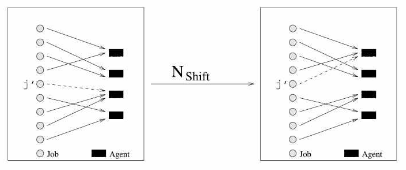
\includegraphics[width=0.7\textwidth]{img/EntornoShift.png}
    \caption{Ejemplo de movimiento shift}
\end{figure}

\newpage

\begin{figure}[h!]
    \centering
    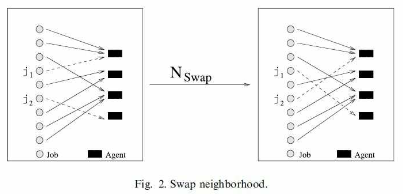
\includegraphics[width=0.7\textwidth]{img/EntornoSwap.png}
    \caption{Ejemplo de movimiento swap}
\end{figure}

\noindent Para obtener una solución mediante busqueda se puede aplicar un único tipo de entorno a la solución ofrecida por el
método Martello-Toth o mezclarlos de forma secuencial o, mejor aún, con un método de descenso VNS.

\subsection{Objetivos minimax}

En algunas ocasiones, tanto en el problema de asignación clásico como en el generalizado, en vez de minimizar el tiempo o 
coste total incurrido al asignar todas las tareas, puede interesar minimizar el tiempo máximo de ejecución entre todas las 
tareas, o bien el tiempo máximo de ejecución entre todas las máquinas. Este segundo objetivo es conocido como 
\textit{makespam}. Aunque ambos objetivos son no lineales, se pueden convertir facilmente en problemas lineales.

\vspace*{2mm}

Para el primer objetivo basta con añadir una variable $w\geq 0$ indicando el tiempo máximo y añadir las restricciones
\[
    \sum_{i=1}^m t_{ij}x_{ij}\leq w \quad j=1,\dots,n
\]

Para el segundo objetivo basta con, de nuevo,  añadir una variable $w\geq 0$ indicando el tiempo máximo y añadir las 
restriciones
\[
    \sum_{j=1}^n t_{ij}x_{ij}\leq w \quad i=1,\dots,m
\]
\section{Problema Bin Packing}

\subsection{Introducción}

El problema de empaquetado de objetos o Problema Bin Packing se produce de forma frecuente en entornos de almacenes,
transporte y mensajería. Los objetos pueden ser paquetes, cajas o pallets\footnote{Se le llama pallet o palé a la plataforma
formada con tablas de madera que se utiliza para el almacenamiento y el traslado de mercancias} que deben ser cargados en 
contenedores, furgonetas, camiones, vagones o cualquier otro medio de transporte. El objetivo es minimizar el coste asociado
al uso de los contenedores, aunque suele reducirse al mínimo de contenedores necesarios para efectuar una carga. Dependiendo
de las características de los objetos se clasifican entre

\begin{itemize}
    \item Problemas de Bin Packing de dimensión uno, para objetos de alta densidad y solo se considera el peso.
    \item Problemas de Bin Packing de dimensión dos, para carga de objetos de la misma altura.
    \item Problemas de Bin Packing de dimensión tres, para carga de objetos de baja densidad, en cuyo caso se considera el
    volumen.
\end{itemize}

\subsection{Problema unidimensional}

Sea $n$ el número de objetos que hay que empaquetar, y para cada $j=1,\dots,n$ $a_j$ es peso del objeto $j$. Se dispone de $m$
contenedores o ``bins'', y para cada $i=1,\dots,m$ $q_i$ es la capacidad o peso total que admite el contenedor $i$ y $c_i$ es
el costo por uso del contenedor $i$. Se supone que todo objeto cabe en el contenedor. Se formula el problema de la siguiente
manera

\begin{alignat}{3}
    \text{minimizar:}   &   \sum_{i=1}^m c_{i}y_{i}               \\
    \text{sujeto a:}    &   \sum_{i=1}^m x_{ij}=1 \quad j=1,\dots,n             \\
                        &   \sum_{j=1}^n a_{j}x_{ij}\leq q_iy_i \quad i=1,\dots,m \\
                        &   x_{ij} \in {0, 1} \quad i=1,\dots,m \quad j=1,\dots,n \\
                        &   y_{i} \in {0, 1} \quad i=1,\dots,m
\end{alignat}

\noindent donde las variables binarias $y_i$ indican el uso del contenedor $i$ y las $x_{ij}$ indican la asignación de objetos
a los contenedores.

Cuando los contenedores son identicos, se toma la capacidad $q_i=q$ para todos los contenedores, y la función objetivo se 
reduce a minimizar el número de contenedores usados
\begin{alignat}{3}
    \text{minimizar:}   &   \sum_{i=1}^m y_{i}
\end{alignat}

\newpage

En algunas ocasiones, el número de contenedores que pueden usarse es ilimitado. Entonces se toma $m$ lo suficietemente grande
para que el modelo tenga solución. Por ejemplo, en el caso de contenedores idénticos basta con que $m=n$, aunque siempre es
preferible un valor menor para que no haya demasidas variables. Para encontrar un valor menor vale con encontrar una solución
factible rápida y usar el número de contenedores utilizados en la solución como valor de $m$.

\subsection{Métodos de solución}

Existen numerosos algoritmos heurísticos para el Problema de Bin Packing, que permiten encontar soluciones factibles cercanas
al óptimo. Por ejemplo, puede aplicarse el algoritmo conocido como FFD (First Fit Decreasing)

\begin{itemize}
    \item \textbf{Etapa 0}. Se ordenan los objetos de forma decreciente respecto del peso. Sea $S$ la lista de objetos, $V$
    la lista de ``bins'' y $T$ la lista de los ``bins'' usados. Inicialmente $T=\emptyset$.
    \item \textbf{Etapa 1}. Elegimos el primer objeto $j$ de la lista $S$ y lo insertamos en el primer ``bin'' $i\in T$ que
    tenga capacidad residual mayor o igual que $a_j$. Si no hay ningún ``bin'' elegimos el primero $k$ de la lista $V$, lo
    añadimos al final de la lista $T$ e insertamos $j$ en $k$.
    \item \textbf{Etapa 2}. Si $S=\emptyset$ se termina, pues todos los objetos han sido ya cargados. Entonces $T$ es el
    conjunto de ``bins'' usados mientras que $V$ son los no usados. Si $S\neq\emptyset$ volvemos a la Etapa 1.
\end{itemize}

\noindent Es posible y sencillo dar una cota de la solución óptima $z$ tal que
\[
    z_1\leq z\leq z_2
\]
\noindent donde $z_2$ es la solución proporcionada por el algoritmo anterior y $z_1$ definida como
\[
    z_1= \ceil*{\frac{\sum_{j=1}^n a_j}{q}}
\]
\noindent En ocasiones resulta ser que $z_1=z_2$, en esta situación hemos encontrado el valor mínimo sin necesidad de
resolver el modelo.

\begin{ejemplo}
    Se tienen que transportar 11 objetos desde un almacén a otro. Los pesos de los objetos vienen dados en la siguiente tabla
    
    \begin{center}
        \begin{tabular}{c|ccccccccccc}
            \hline
            objeto & 1 & 2 & 3 & 4 & 5 & 6 & 7 & 8 & 9 & 10 & 11 \\ \hline
            peso & 67.3 & 504 & 121 & 130 & 375 & 234 & 73.7 & 175 & 8.5 & 225 & 50.5 \\ \hline
        \end{tabular}
    \end{center}

    Los objetos deben ser transportados en furgonetas que admiten hasta 670 Kg (es decir, $q=670$). El algoritmo FFD encuentra
    una asignación de los 11 objetos a 3 furgonetas, por tanto $z_2=3$. Como $z_1=\ceil*{\frac{\sum_{j=1}^n a_j}{q}}=
    \ceil*{\frac{1964}{670}}=\ceil*{2.93}=3$, en este caso podemos asegurar que el mínimo número necesario de furgonetas es 3.
\end{ejemplo}

\section{Problemas de Diseño de Redes}

\subsection{Introducción}

Los problemas de diseño de redes constituyen un área de problemas donde se tiene que encontrar la configuración o el diseño
óptimo de una red, de forma que se cumplan ciertos criterios de servicio y conectividad, dependiendo del problema concreto.
Este área tiene muchas aplicaciones prácticas, fundamentalmente en problemas de redes de comunicaciones y en redes logísticas
de distribución. Cuando el objetivo no es el diseño de la red sino la optimización del uso de la misma se tienen los problemas
de optimización de flujo en red. En la siguiente tabla se muestran ejemplos de problemas de cada tipo

\begin{table}[h!]
    \centering
    \begin{tabular}{l|l}
        \textbf{Problemas de optimización del uso} & \textbf{Problemas de diseño} \\ \hline
        Problemas de transporte & Problemas de localización con costos fijos \\
        Flujo en redes de un producto & Transporte con costos fijos \\
        Flujo en redes multiproducto & Flujo en redes con costes fijos \\
        Transporte en dos etapas & Sistema de distribución en dos etapas
    \end{tabular}
\end{table}

\subsection{Sistemas de distribución}

Los problemas de planificación de la distribución de productos se clasifican en tres tipos, problemas estratégicos (plazo
largo, incertidumbre grande), problemas tácticos (plazo medio, incertidumbre menor) y problemas operacionales (plazo muy
corto, incertidumbre pequeña). Para el diseño de un sistema de distribución de productos hay 3 esquemas o sistemas básicos

\begin{itemize}
    \item \textbf{Transporte directo}. Los productos se transportan directamente desde las plantas hasta los puntos de
    distribución finales. El problema de diseño para este tipo de sistema para un único producto se modela como un problema
    de localización con costes fijos en una de sus tres variantes, UFLP (Uncapacited Facility Location Problem), CFLP
    (Capacited Facility Location Problem) o SSCFLP (Single Source Capacitated Facility Location Problem). La optimización de
    un sistema ya diseñado se reduce al problema de transporte clásico.
    \item \textbf{Almacenamiento}. Es el método tradicional de almacenar los productos en tanques/almacenes intermedios. El problema de
    optimización para un producto es un problema de transporte en dos etapas que tambien puede modelizarse como problema de
    flujo en redes.
    \item \textbf{Terminales de carga (Crossdocking)}. Este método se conoce tamién como distribución just-in-time. Los
    productos se envían a una instalación ``crossdock'' con terminales de carga donde son ordenados, las cargas se consolidan
    con otros productos y se envian con trailers a los puntos de demanda sin necesidad de almacenarlos. El problema de
    optimización de un sistema con terminales de carga es un problema de flujos en redes multiproducto, y el problema de diseño
    es un problema de flujos en redes multiproductos con costos fijos.
\end{itemize}

\subsection{Problema de Flujo en Redes con Costos Fijos (FCNP)}

Se tiene un grafo dirigido $G=(N,A)$ con $N=\{1,\dots,n\}$ conjunto de nodos y $A$ un conjunto de arcos, donde cada arco
corresponde a un par $(i,j)$ tal que $i,j\in N$. Asociado a cada arco hay una variable de flujo con valores 
$0\leq x_{ij}\leq u_{ij}$ donde $u_{ij}$ es una cota superior del flujo en el arco $(i,j)$ y una variable binaria 
$y_{ij}\in\{0,1\}$ que representa el ``uso'' del arco en la solución final (cuando $x_{ij}>0$).Para ello es necesaria la
restricción
\[
    x_{ij}\leq u_{ij}y_{ij}
\]
Las variables $y_{ij}$ son las variables de diseño y tienen asociadas en la función objetivo un costo fijo $f_{ij}$. En 
ocasiones las variables $x_{ij}$ tienen asociado un costo variable $c_{ij}$. Finalmente, $b_i$ es la oferta o demanda del
nodo $i$. Se formula el modelo, suponiendo la red balanceada, como

\begin{alignat}{3}
    \text{minimizar:}   & \sum_{(i,j)\in A}(f_{ij}y_{ij} + c_{ij}x_{ij})    &                       \\
    \text{sujeto a:}    & \sum_{j=1}^nx_{ij}-\sum_{j}x_{ji}=b_i                 & \forall i\in N        \\
                        & x_{ij}\leq u_{ij}y_{ij}                           & \forall (i,j)\in A    \\
                        & x_{ij}\geq 0                                      & \forall (i,j)\in A    \\
                        & y_{ij}\in\{0,1\}                                  & \forall (i,j)\in A
\end{alignat}

\subsection{Problema Conector}

El Problema Conector consiste en encontar la forma de conectar $n$ puntos (nodos) entre si con costo o distancia total mínima 
a partir de un árbol $G=(N,A)$ donde cada arista $(i,j)$ tiene asociado un costo $\omega_{ij}$. Un subgrafo expandido conexo 
es un grafo $G'=(N,T)$, con conjunto de aristas $T\subseteq A$ que conecta entre si todos los nodos de $N$, y que tiene 
asociado un costo total $\omega(T)=\sum_{(i,j)\in T}\omega_{ij}$. El problema conector se reduce a encontrar el subgrafo 
expandido conexo de menor costo total.

\subsubsection{Minimum Spaning Tree (MST)}

Un árbol es un grafo conexo y sin ciclos. En la mayoria de problemas prácticos de conexión se puede suponer que 
$\omega_{ij}>0$ para toda arista $(i,j)\in A$. En este caso el Problema Conector tiene como solución un árbol expandido,
pues si existiese un grafo expandido con algún ciclo simplemente se puede eliminar una arista manteniendo la conexión entre
todos los nodos y reduciendo \textbf{siempre} el costo total. 

Por tanto el Problema Conector se ve reducido al problema MST (Minimun Spanning Tree), que puede ser formulado como Problema 
de Flujo en Redes con Costos Fijos. Primero se duplica cada arísta en dos arcos, pues el Problema de Flujo en Redes con Costos
Fijos es dirigido, $i\to j$ y $j\to i$. Si se van a conectar $n$ puntos, se elige uno arbitariamente (nodo $k$) y se toman 
ofertas/demandas de $b_k=n-1$ y $b_i=-1$ para $k\neq i$. Estas ofertas y demandas obligan a conectar todos los puntos 
proporcionando una solución de grafo conexo. En la función objetivo solo aparecerán los costos de los arcos por las variables 
de diseño binarias $y_{ij}$ (no hay costos variables). Por último, para asociar las variables 
$x_{ij}\geq 0$ y $y_{ij}\in\{0,1\}$ en las restricciones $x_{ij}\leq u_{ij}y_{ij}$ se puede usar como $u_{ij}=n-1$ para todo 
arco $(i,j)\in A$.

\vspace*{2mm}

A pesar de que el problema MST puede ser formulado como problema mixto de redes con costes fijos, hay algoritmos que lo
resuelven fácilmente sin necesidad de plantear el modelo.

\newpage

\subsubsection{Algoritmo de Kruskal}

Es un caso particular de los algoritmos ``greedy'' pues en cada paso se toma la arista o variable de costo mínimo, y no se
vuelve a reoptimizar o corregir. Para el MST el algoritmo es el siguiente

\begin{itemize}
    \item \textbf{Etapa inicial}. Se elige una arista de costo mínimo
    \item \textbf{Etapa general}. Si se han elegido ya aristas $A'=\{a_1,\dots,a_i\}$ se elige la siguiente arista 
    $a_{1+1}\in A-A'$ de forma que se verifique que en $A'=\{a_1,\dots,a_i,a_{i+1}\}$ no hay ciclos y el costo 
    $\omega(a_{i+1})$ es mínimo.
    \item \textbf{Etapa final}. Se termina cuando ya no se pueda realizar la etapa anterior (siempre en $n-1$ etapas).
\end{itemize}

\subsubsection{Algoritmo de Prim}

Se trata de otra implementación del algoritmo greedy. En vez de ir añadiendo aristas hasta formal el árbol final (con las 
comprobaciones de ciclos que conlleva), en este método se va aumentando un árbol expandido $T_j$ desde uno con un único nodo y
ninguna arista hasta uno con $n$ nodos y $n-1$ aristas.

\begin{itemize}
    \item \textbf{Etapa inicial}. $T_0$ consiste de un único nodo.
    \item \textbf{Etapa general}. Dado $T_{j-1}$ árbol conteniendo $j$ nodos y $j-1$ aristas, se añadie la arista de costo o
    peso mínimo entre todas las aristas con un extremo en $T_{j-1}$ y otro en $T_{j-1}'$.
    \item \textbf{Etapa final}. Se termina con el árbol $T_{n-1}$ (siempre en $n-1$ etapas).
\end{itemize}

\subsubsection{Capacitated Minimum Spaning Tree (CMST)}

El Problema del Mínimo Árbol con Capacidades (CMST) es una versión del problema MST con la concición adicional de que ninguno
de los sub-árboles saliendo desde la raíz tenga más de $k$ nodos. Salvo para los casos triviales de $k=1$ (árbol estrella) y 
$k\geq n-1$ (MST) se trata de un problema mucho más dificil de resolver que el MST y no existe ningún algoritmo simple
(polinómico) pàra su resolución.


En otra versión del problema existen demandas $d_i$ desde los nodos $i\neq 1$ al nodo raíz o desde el nodo raíz al resto de
nodos. En este caso la restricción de capacidad es un límite $C$ sobre la capacidad de tráfico que puede manejar. Entonces se
debe cumplir la restricción $\sum_{i\in T_k}d_i \leq C$ donde $T_k$ es el conjunto de nodos del árbol conectado a cualquier
puerto $k$.

\vspace*{2mm}

El problema CMST se puede formular como un Problema de Flujo en Redes con Costos Fijos con las siguientes características.
\begin{enumerate}
    \item Costos fijos. $f_{ij}=\omega_{ij}$ mientras que los costos variables son nulos para todo arco $(i,j)\in A$.
    \item Ofertas/demandas. Hay dos formas de formularlas, dependiendo de si el flujo es de los nodos a la raíz $r$ o de la 
    raíz a los nodos. Si el tráfico es de los nodos a la raíz, en el modelo de redes se toman como ofertas/demandas $b_i=1$
    para $i\neq r$ y $b_r=-(n-1)$, y para el caso de demandas de tráfico $b_i=d_i$ para $i\neq r$ y $b_r=-\sum d_r$. Cuando el
    tráfico es de la raíz a los nodos se toman como ofertas/demandas $b_i=-1$ para $i\neq r$ y $b_r=(n-1)$, y para el caso de
    demandas $b_i=-d_i$ para $i\neq r$ y $b_r=\sum d_r$. En todos los casos la red está balanceada.
    \item Capacidades. En el caso del tráfico de los nodos a la raíz, $u_ir=k$ y para el resto en principio no hay restricción
    de capacidad. Si el tráfico va del nodo raíz hasta el resto de nodos, $u_ri=k$ y para el resto no hay restricción de
    capacidad.
\end{enumerate}

\newpage

\subsubsection{Métodos heurísticos CMST}

Existe uma variedad de métodos heurísticos para el problema CMSP. Heurísticas de construcción conocidas son la heurística de
Eseau-Williams, que tiene su origen en el conocido algoritmo de Clarke-Wright para el problema de rutas con capacidades y se
basa en el concepto de ahorro (saving). Otra más sencilla es el algoritmo de Prim modificado, el método consiste en ir
construyendo subárboles con raíz en el nodo base $r$, con el criterio del método greedy de Prim y respetando la restricción
de capacidad (se puede realizar de forma secuencial o en paralelo).

\subsubsection{Problema de Steiner}

Otro Problema Conector que surge en la práctica es el Problema de Steiner. En este problema se tiene, al igual que en el MST,
un grafo $G=(N,A)$ con pesos o distancias en las aristas $\omega_{ij}$ para $(i,j)\in A$ y uin subconjunto de nodos
$T\subseteq N$ conocidos como terminales. El problema consiste en encontrar un subgrafo que conecte los nodos terminales entre
sí y que tenga peso total mínimo. Si los pesos son positivos la solución final tendrá forma de árbol, conocido como árbol de
Steiner. Si $T=N$ el problema se reduce al MST, mientras que si $|T|=2$ se reduce al del camino más corto entre los dos nodos
en $T$. Para el resto de casos, el problema de Steiner es un problema dificil para el que no existe ningún algoritmo
polinómico.

El problema del mínimo árbol de Steiner se puede formular como un problema de flujo en redes con costos fijos con las siguientes
características

\begin{enumerate}
    \item Se transforma el grafo en uno dirigido duplicando cada arista $(i,j)$ en dos arcos dirigidos $(i,j)$ y $(j,i)$.
    \item Costos fijos. $f_{ij}=\omega_{ij}$ mientras que los costos variables son nulos para todo arco $(i,j)\in A$.
    \item Ofertas/demandas. Se escoge arbitrariamente un nodo terminal como raíz $r\in T$ y se toman como ofertas/demandas
    $b_r=|T|-1$ y $b_i=-1$ para $i\in T$, $i\neq r$ y $b_i=0$ para todo $i\notin T$.
    \item Capacidades. Las capacidades de los arcos se toman igual al flujo total, que es $|T|-1$.
\end{enumerate}

\subsection{Modelos de Diseño Redes Multiproducto con Costos Fijos}

Los problemas de diseño de redes multiproducto son una extensión a varios productos de los problemas de diseño vistos
anteriormente. Los elementos básicos son un grafo dirigido $G=(N,A)$ donde $N$ es el conjunto de nodos y $A$ el conjunto de
arcos, y un conjunto de productos $K$. En los siguientes modelos tenemos de nuevo dos clases de variables de decisión, la
cantidad de flujo del producto $k$ que pasa por el arco $(i,j)$ que denotaremos como $x_{ij}^k$ y $y_{ij}$ que indican si el
arco $(i,j)$ se usa o no en el diseño solución. Para cada $x_{ij}^k$ tendremos un coste unitario $c_{ij}^k$ asociado y en el
caso de las $y_{ij}$ un coste fijo $f_{ij}$. También hay una serie de ofertas/demandas $b_i^k$ para cada nodo $i\in N$.

\begin{flushright}
    Hasta aquí llegué, consultar más en los apuntes que me va a dar un chungazo de escribír\footnote{Es mucho y repetitivo de 
    anteriores temas pero generalizado a $K$ productos, consultar en el document ``Diseño redes multiproducto.pdf. Más adelante
    esta sección será completada correctamente. La formula objetivo y las restricciones son bastante sencillas de intuir.''}
\end{flushright}
\section{Modelos de Localización}

\subsection{Introducción}

Los problemas de Localización constituyen uno de los grupos de problemas de Investigación Operativa que más se han aplicado en
la práctica. La característica común a todos ellos es la necesidad de situar algún objeto o instalación de la mejor manera
posible. Si los lugares donde pueden estar situados estos objetos están restringidos a un conjunto discreto (generalmente
infinito) estaríamos dentro de la \textit{localización discreta}, que es la que se va a tratar aquí.

En muchos problemas se tienen los siguientes elementos básicos. Hay $m$ puntos de demanda de cierto servicio que hay que
cubrir, y $n$ posibles puntos donde situar una ``instalación'' o punto de servicio. El problema es decidir el número y la
localización de los puntos de servicio de forma que se optimice cierto objetivo, que suele depender de los costos de
instalación y de los costos del servicio. Según los objetivos que se consideren se tienen los siguientes problemas básicos
de localización

\begin{itemize}
    \item Problemas de Cubrimiento Total (Set Covering).
    \item Problemas de Cubrimiento Máximo.
    \item Problemas de Localización de Midianas.
    \item Problemas de Localización de Centros de Emergencia.
    \item Problemas de Localización con Costos Fijos.
    \item Problemas de Distritos.
\end{itemize}

\noindent Se van a describir los Problemas de Localización con Costos Fijos básicos.

\subsection{Problema de Localización con Costos Fijos}

Sea $M=\{1,\dots,m\}$ el conjunto de los puntos de demanda de cierto servicio y $N=\{1,\dots,n\}$ el conjunto de puntos donde
puede estar situada la instalación. En este tipo de modelos se supone que cada punto de demanda $i\in M$ tiene una demanda
$d_i$ de cierto servicio y que para $j\in N$ hay un coste fijo $f_j$ de apertura o mantenimiento de la instalación. Además,
se tiene un costo variable o unitario $c_{ij}$ asociado a servir una unidad de demanda al cliente $i$ desde la instalación
$j$. Si suponemos que las instalaciones pueden servir cualquier cantidad de demanda se tiene el Modelo de Localización sin
Capacidades, que se formula tal que

\begin{alignat}{3}
    \text{minimizar:}   & \sum_{j=1}^n(f_{j}x_{j} + \sum_{i=1}^m\sum_{j=1}^n c_{ij}z_{ij})  &                           \\
    \text{sujeto a:}    & \sum_{j=1}^nz_{ij}=d_i                                            & i=1,\dots,m               \\
                        & \sum_{i=1}^nz_{ij}\leq Mx_j                                       & j=1,\dots,n               \\
                        & z_{ij}\geq 0                                                      & i=1,\dots,m\; j=1,\dots,n \\
                        & x_{j}\in\{0,1\}                                                   & j=1,\dots,n
\end{alignat}

\noindent donde $x_j$ son las variables de localización binarias, corresponden a las decisiones de apertura o no de las
instalaciones y $z_{ij}$ indican las cantidades que se sirven desde cada instalación hasta cada cliente o punto de demanda.

\vspace*{2mm}

Haciendo el cambio de variable $y_{ij}=\frac{z_{ij}}{d_i}$ la variable $y_{ij}$ indica la fracción de la demanda del cliente
$i$ cubierta desde la instalación $j$ quedando un modelo más comunmente usado tal que

\begin{alignat}{3}
    \text{minimizar:}   & \sum_{j=1}^n(f_{j}x_{j} + \sum_{i=1}^m\sum_{j=1}^n c_{ij}y_{ij}d_i)   &                           \\
    \text{sujeto a:}    & \sum_{j=1}^ny_{ij}=1                                                  & i=1,\dots,m               \\
                        & \sum_{i=1}^ny_{ij}\leq mx_j                                           & j=1,\dots,n               \\
                        & 0\leq y_{ij}\leq 1                                                    & i=1,\dots,m\; j=1,\dots,n \\
                        & x_{j}\in\{0,1\}                                                       & j=1,\dots,n
\end{alignat}

\noindent donde ahora ya no es preciso un $M$ lo suficientemente grande sino que vale con $m$ el número de puntos demanda. 

\vspace*{2mm}

Si para cada posible instalación $j\in N$ hay una capacidad $u_j$ para la demanda total que puede servir, se tiene el modelo 
de Localización con Capacidades siguiente

\begin{alignat}{3}
    \text{minimizar:}   & \sum_{j=1}^n(f_{j}x_{j} + \sum_{i=1}^m\sum_{j=1}^n c_{ij}y_{ij}d_i)   &                           \\
    \text{sujeto a:}    & \sum_{j=1}^ny_{ij}=1                                                  & i=1,\dots,m               \\
                        & \sum_{i=1}^nd_iy_{ij}\leq u_jx_j                                      & j=1,\dots,n               \\
                        & 0\leq y_{ij}\leq 1                                                    & i=1,\dots,m\; j=1,\dots,n \\
                        & x_{j}\in\{0,1\}                                                       & j=1,\dots,n
\end{alignat}

\noindent conocida como formulación débil. Añadiendo la restricción $y_{ij}\leq x_j$ para $j=1,\dots,n$ se refuerza
considerablemente la relajación lineal del problema, conocida como formulación fuerte.

En una variante de estos modelos se exige que cada punto de demanda será cubierto por una única instalación. Esta restricción
se conoce como de fuente única. En el caso del modelo sin capacidades la solución óptima siempre puede tomarse verificando
esta condición, pues al no haber capacidades, cada punto de demanda será servido por la instalación abierta más cercana. 

\newpage

Sin embargo, en el caso capacitado lo anterior ya no puede garantizarse y se obtiene así el modelo conocido como Modelo de
Localización con Capacidades y Fuente Única (SSCFL) siguiente

\begin{alignat}{3}
    \text{minimizar:}   & \sum_{j=1}^n(f_{j}x_{j} + \sum_{i=1}^m\sum_{j=1}^n c_{ij}y_{ij}d_i)   &                           \\
    \text{sujeto a:}    & \sum_{j=1}^ny_{ij}=1                                                  & i=1,\dots,m               \\
                        & \sum_{i=1}^nd_iy_{ij}\leq u_jx_j                                      & j=1,\dots,n               \\
                        & y_{ij}\in\{0,1\}                                                      & i=1,\dots,m\; j=1,\dots,n \\
                        & x_{j}\in\{0,1\}                                                       & j=1,\dots,n
\end{alignat}

\noindent donde tanto $x_j$ como $y_{ij}$ son variables binarias. El modelo es considerablemente más dificil de resolver que
el CFL normal, y generalmente debe recurriste al uso de heurísticas para su resolución aproximada.

\subsection{Algoritmo greedy ADD para UFLP}

Al enfrentar la evolución del coste fijo, coste por unidad y el coste total contra el número de instalaciones se obtiene el
siguiente gráfico

\begin{center}
    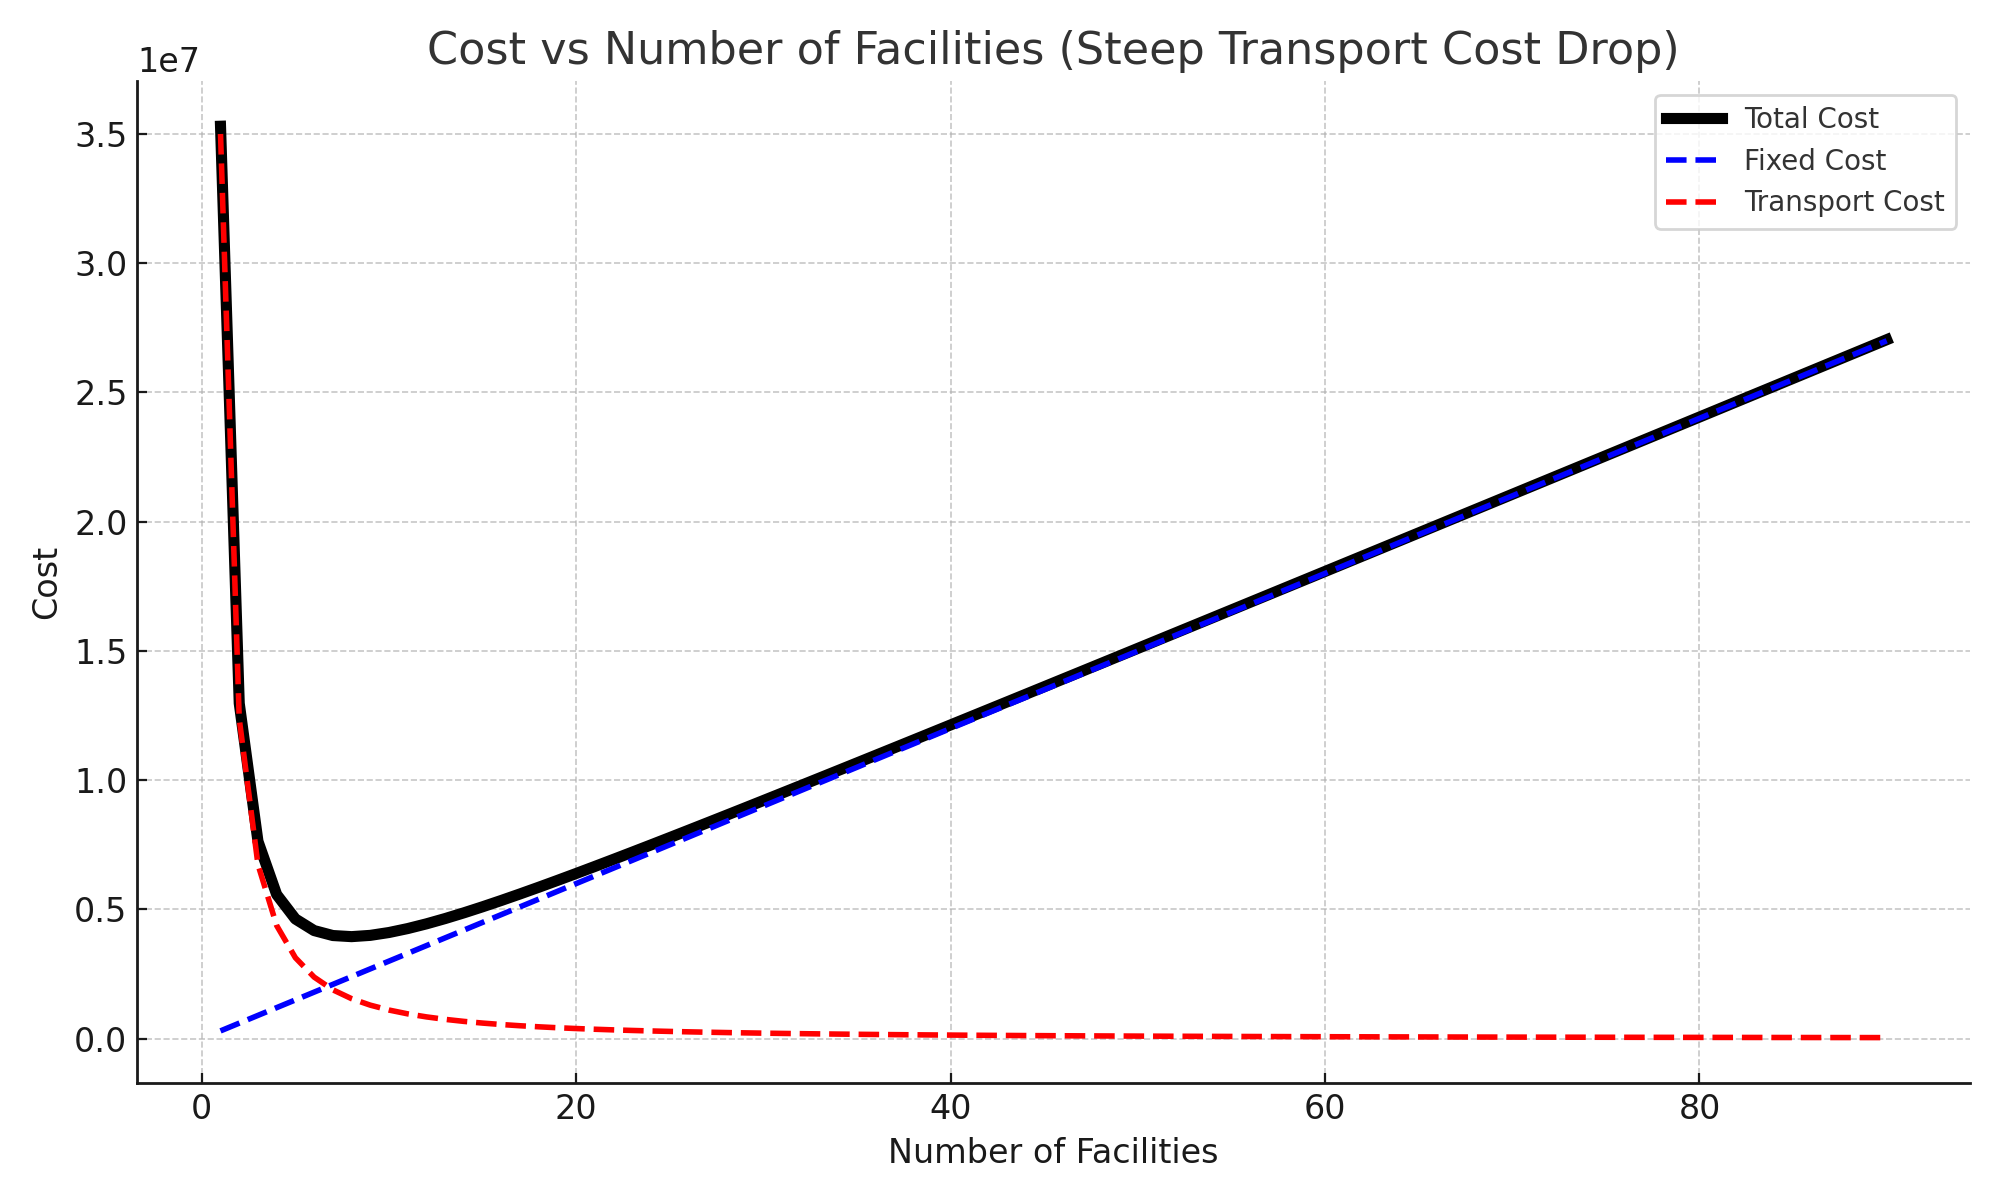
\includegraphics[width=0.8\textwidth]{img/GraficoCosteCentros.png}
\end{center}

\noindent se aprecia que existe un punto donde se minimiza el coste total justo donde se cruzan la función coste fijo y la
función coste por unidad. Esta propiedad la aprovechan los algoritmos greedy ADD y DROP para encontrar una solución factible
cercana al óptimo.

\vspace*{2mm}

Con el método ADD comenzamos en el lado izquierdo de la curva con una única instalación y se van añadiendo instalaciones de
dorma greedy mientras el costo total va disminuyendo (mayor decrecimiento y menor costo) y no se modifican elecciones hechas
hasta ese momento. Si no es posible mejorar añadiendo ninguna fabrica más hemos encontrado la solución.

Con el método DROP, se comienza en el lado derecho de la curva abriendo todas las intalaciones posibles y se van cerrando una
a una de forma greedy mientras el costo total disminuya.

Estos métodos fueron diseñados originalmente para el problema sin capacidades, y posteriormente se han extendido a muchos
otros problemas de localización. Para el problema UFLP se usan las siguientes notaciones. $z^h$ es el valor heurístico de la
solución actual y $S\subseteq N$ es el subconjunto de instalaciones abiertas. De forma equivalente, en lugar de $S$ puede
darse el array $x=(x_j)$ para $j=1,\dots,n$ donde $x_j=1$ si $j\in S$ y 0 en otro caso. Para el problema UFL es suficiente
representar la solución mediante el subconjunto $S\subseteq N$ o el array $x$, pues cada punto de demanda $i$ se asignará al 
punto de servicio abierto más cercano. Esto podemos darlo en otro array $y=(y_i)$ para $i=1,\dots,m$ con las asignaciones
actuales, es decir, $y_i$ es el punto de servicio abierto que sirve al punto de demanda $i$.

\subsection{Heurísticas de mejora para UFL}

Se parte de la solución factible obtenida con alguno de los procedimientos ADD o DROP de la sección anterior. Como a priori no
conocemos el número total de instalaciones o puntos de servicio que pueden ser abiertos en una solución óptima, los métodos de
mejora deben incluir la posibilidad de cerrar una instalación abierta (método drop), de abrir o añadir una nueva instalación
(método add), y también un posible intercambio (método swap), que consistiría en cerrar una y abrir otra simultaneamente.
Combinando estos métodos podemos generar entornos de solución sobre los que realizar busqueda local y aproximarnos a la
solución óptima.

\newpage

% ------------------------------------------------------------------------------
% Reference and Cited Works
% ------------------------------------------------------------------------------

\begin{thebibliography}{9}
    \bibitem{PDFs}
    José Ignacio Segovia Martín, Ricardo Josa Fombellida, \\ \textit{PDF de la asignatura PENT}. \\ Universidad de Valladolid 2024.
\end{thebibliography}

% ------------------------------------------------------------------------------

\end{document}
